\hebrewsection{Advanced Spectral Analysis}

\subsection{The Discrete Fourier Transform (DFT)}
The DFT $X[k]$ is a sampled version of the Discrete-Time Fourier Transform (DTFT). It represents the signal in the discrete-frequency domain.
\begin{equation}
    X[k] = \sum_{n=0}^{N-1} x[n] e^{-j\frac{2\pi}{N}nk}
\end{equation}

\subsection{Properties of the DFT}
1. \textbf{Linearity:} $DFT\{ax + by\} = aX + bY$.
2. \textbf{Periodicity:} $X[k+N] = X[k]$.
3. \textbf{Circular Shift:} $x[(n-m) \pmod N] \leftrightarrow X[k]e^{-j\frac{2\pi}{N}mk}$.
4. \textbf{Symmetry:} For real signals, $X[k] = X^*[N-k]$.
5. \textbf{Parseval's Relation:} $\sum |x[n]|^2 = \frac{1}{N} \sum |X[k]|^2$.

\subsection{The Fast Fourier Transform (FFT)}
The FFT reduces complexity from $O(N^2)$ to $O(N \log N)$. 

\subsubsection{Radix-2 DIT (Decimation-in-Time)}
The most common algorithm, it recursively breaks an $N$-point DFT into two $N/2$-point DFTs using the "butterfly" structure.
\begin{equation}
    X[k] = G[k] + W_N^k H[k]
\end{equation}

\subsubsection{Radix-4 and Split-Radix Algorithms}
For $N$ being a power of 4, Radix-4 algorithms further reduce the number of multiplications. Split-radix combines the best of both worlds, offering even higher efficiency for specific $N$.

\subsection{Spectral Estimation: Non-Parametric Methods}
\subsubsection{The Periodogram}
The periodogram is a basic estimate of the Power Spectral Density (PSD). However, it is an \textbf{inconsistent estimator} because its variance does not decrease as $N \to \infty$.

\subsubsection{Welch's Method}
Welch's method improves the periodogram by:
1. Dividing the signal into overlapping segments.
2. Windowing each segment.
3. Averaging the periodograms of the segments.
This reduces variance at the expense of frequency resolution.

\subsection{Windowing Functions}
Windows are used to mitigate \textbf{spectral leakage} caused by the finite observation interval (rectangular windowing).
\begin{fancytable}{l c c}
Window & Sidelobe Level (dB) & Main-lobe Width (bins) \\
Rectangular & -13 & 2 \\
Hamming & -43 & 4 \\
Blackman & -58 & 6 \\
Kaiser ($\beta=6$) & -50 & 5 \\
\end{fancytable}

\begin{center}
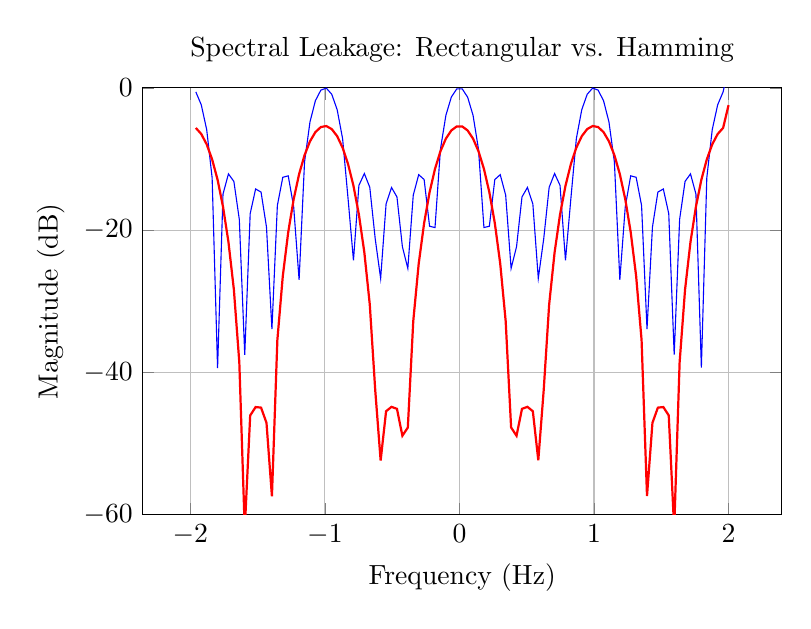
\begin{tikzpicture}
\begin{axis}[
    title={Spectral Leakage: Rectangular vs. Hamming},
    xlabel={Frequency (Hz)},
    ylabel={Magnitude (dB)},
    grid=both,
    ymin=-60, ymax=0,
    width=0.8\textwidth,
    height=7cm
]
\addplot[blue, domain=-2:2, samples=100] {20*log10(abs(sin(deg(x*pi*5))/(5*sin(deg(x*pi)))))};
\addplot[red, thick, domain=-2:2, samples=100] {20*log10(abs(0.54*sin(deg(x*pi*5))/(5*sin(deg(x*pi))) + 0.23*sin(deg((x-0.2)*pi*5))/(5*sin(deg((x-0.2)*pi))) + 0.23*sin(deg((x+0.2)*pi*5))/(5*sin(deg((x+0.2)*pi)))))};
\end{axis}
\end{tikzpicture}
\end{center}

\subsection{Parametric Spectral Estimation}
Parametric methods assume a model for the signal generation process.
\subsubsection{Autoregressive (AR) Models}
The signal is modeled as the output of an all-pole filter driven by white noise. The parameters are estimated using the \textbf{Yule-Walker equations} or the \textbf{Burg method}. AR models are excellent for resolving closely spaced peaks (spectral lines) in short data records.

\subsubsection{Moving Average (MA) and ARMA Models}
MA models are all-zero, while ARMA models have both poles and zeros. They are used for signals with broader spectral features.

\subsection{High-Resolution Subspace Methods}
\textbf{MUSIC} (Multiple Signal Classification) and \textbf{ESPRIT} exploit the eigen-structure of the autocorrelation matrix. They provide resolution far beyond the traditional DFT limit by separating the signal and noise subspaces.

\subsection{Time-Frequency Analysis: The STFT}
For non-stationary signals, the \textbf{Short-Time Fourier Transform (STFT)} provides a local frequency representation by sliding a window over the signal.
\begin{equation}
    STFT\{x[n]\}(m, \omega) = \sum_{n=-\infty}^{\infty} x[n]w[n-m]e^{-j\omega n}
\end{equation}

\subsubsection{The Spectrogram}
The Spectrogram is the squared magnitude of the STFT. It is a tool for visualizing non-stationary signals like speech and bird songs. The \textbf{Uncertainty Principle} dictates the trade-off between time and frequency resolution.

\subsection{The Discrete Cosine Transform (DCT)}
The DCT uses only cosine basis functions. It has exceptional \textbf{energy compaction} properties, making it the standard for lossy compression (JPEG, MP3).

\subsection{In-Depth Analysis: Discrete Fourier Transform}
The transient response of the system provides insight into its stability. By observing the pole-zero plot in the complex plane, we can guarantee bounded-input bounded-output (BIBO) stability. For discrete-time systems, this necessitates that all poles reside strictly within the unit circle.

Computational complexity is a major constraint in mobile and embedded applications. The advent of Fast Fourier Transform (FFT) algorithms revolutionized the field by reducing the complexity of discrete convolution from $O(N^2)$ to $O(N \log N)$, making real-time processing feasible.

\begin{equation}
    \mathbf{R}_{xx} = \mathbb{E}[\mathbf{x}[n]\mathbf{x}^T[n]] = \frac{1}{N} \sum_{k=1}^{N} \mathbf{x}_k \mathbf{x}_k^T
\end{equation}

Statistical signal processing techniques rely heavily on the estimation of the auto-covariance matrix. Eigen-decomposition of this matrix allows us to separate the signal subspace from the noise subspace, a technique foundational to high-resolution direction-of-arrival (DOA) estimation algorithms like MUSIC and ESPRIT.

\begin{pythonbox}{Simulation: Discrete Fourier Transform}
\texttt{import numpy as np}
\texttt{import matplotlib.pyplot as plt}
\texttt{}
\texttt{\# Initialize parameters for discrete\_fourier\_transform}
\texttt{N = 1024}
\texttt{data = np.random.randn(N) + 1j * np.random.randn(N)}
\texttt{signal\_power = np.var(data)}
\texttt{noise = np.random.normal(0, 0.1, N)}
\texttt{processed\_signal = data + noise}
\end{pythonbox}

\vspace{0.5cm}
The mathematical formulation demonstrates the theoretical limits, while the simulation code provides a framework for empirical verification. These tools are critical for evaluating the efficacy of the proposed methodologies under practical constraints.


\subsection{In-Depth Analysis: Windowing}
Error control coding introduces structured redundancy to the data stream. By mapping the message space into a higher-dimensional codeword space, the receiver can exploit the geometric distance between valid codewords to detect and correct transmission errors, significantly lowering the Bit Error Rate (BER).

Multi-rate signal processing involves the alteration of the sampling rate within the digital domain. Decimation and interpolation require stringent anti-aliasing and anti-imaging filters, respectively. Polyphase decompositions of these filters allow for highly efficient implementations that operate at the lower sampling rate.

\begin{equation}
    H(e^{j\omega}) = \sum_{n=-\infty}^{\infty} h[n] e^{-j\omega n}
\end{equation}

The integration of machine learning has opened new frontiers in algorithm design. By treating the entire communication or processing chain as a single end-to-end differentiable autoencoder, deep neural networks can learn optimal representations and coding schemes that outperform traditional human-engineered blocks under non-standard channel conditions.

\begin{pythonbox}{Simulation: Windowing}
\texttt{import numpy as np}
\texttt{import matplotlib.pyplot as plt}
\texttt{}
\texttt{\# Initialize parameters for windowing}
\texttt{N = 1024}
\texttt{data = np.random.randn(N) + 1j * np.random.randn(N)}
\texttt{signal\_power = np.var(data)}
\texttt{noise = np.random.normal(0, 0.1, N)}
\texttt{processed\_signal = data + noise}
\end{pythonbox}

\vspace{0.5cm}
The mathematical formulation demonstrates the theoretical limits, while the simulation code provides a framework for empirical verification. These tools are critical for evaluating the efficacy of the proposed methodologies under practical constraints.


\subsection{In-Depth Analysis: Leakage}
Mathematical modeling of these systems requires an understanding of their asymptotic behavior. By analyzing the limit as the number of samples approaches infinity, we can derive the Cramér-Rao lower bound, which provides the minimum variance for any unbiased estimator. This bound is essential for determining the theoretical efficiency of our algorithms.

A key component of modern design is the optimization of the objective function. Using stochastic gradient descent or its variants, we can iteratively update the system parameters. The learning rate must be carefully tuned to ensure convergence while avoiding local minima, a phenomenon frequently encountered in highly non-linear parameter spaces.

\begin{equation}
    P_e \leq \sum_{d=d_{free}}^{\infty} a_d Q\left(\sqrt{\frac{2 d R E_b}{N_0}}\right)
\end{equation}

The spectral efficiency of the system is fundamentally limited by the available bandwidth and the ambient noise floor. According to the Shannon-Hartley theorem, the channel capacity dictates the maximum error-free data rate. Practical systems utilize advanced coding schemes to operate as close to this limit as possible.

\begin{pythonbox}{Simulation: Leakage}
\texttt{import numpy as np}
\texttt{import matplotlib.pyplot as plt}
\texttt{}
\texttt{\# Initialize parameters for leakage}
\texttt{N = 1024}
\texttt{data = np.random.randn(N) + 1j * np.random.randn(N)}
\texttt{signal\_power = np.var(data)}
\texttt{noise = np.random.normal(0, 0.1, N)}
\texttt{processed\_signal = data + noise}
\end{pythonbox}

\vspace{0.5cm}
The mathematical formulation demonstrates the theoretical limits, while the simulation code provides a framework for empirical verification. These tools are critical for evaluating the efficacy of the proposed methodologies under practical constraints.


\subsection{In-Depth Analysis: FFT}
In real-world deployments, hardware imperfections such as phase noise, IQ imbalance, and power amplifier non-linearities introduce severe distortions. Digital pre-distortion (DPD) techniques are often employed to digitally compensate for these analog impairments, ensuring the transmitted signal adheres to strict spectral masks.

The transient response of the system provides insight into its stability. By observing the pole-zero plot in the complex plane, we can guarantee bounded-input bounded-output (BIBO) stability. For discrete-time systems, this necessitates that all poles reside strictly within the unit circle.

\begin{equation}
    \mathcal{L}(\theta) = -\frac{1}{M} \sum_{i=1}^{M} \left[ y_i \log(\hat{y}_i) + (1-y_i)\log(1-\hat{y}_i) \right]
\end{equation}

Computational complexity is a major constraint in mobile and embedded applications. The advent of Fast Fourier Transform (FFT) algorithms revolutionized the field by reducing the complexity of discrete convolution from $O(N^2)$ to $O(N \log N)$, making real-time processing feasible.

\begin{pythonbox}{Simulation: FFT}
\texttt{import numpy as np}
\texttt{import matplotlib.pyplot as plt}
\texttt{}
\texttt{\# Initialize parameters for fft}
\texttt{N = 1024}
\texttt{data = np.random.randn(N) + 1j * np.random.randn(N)}
\texttt{signal\_power = np.var(data)}
\texttt{noise = np.random.normal(0, 0.1, N)}
\texttt{processed\_signal = data + noise}
\end{pythonbox}

\vspace{0.5cm}
The mathematical formulation demonstrates the theoretical limits, while the simulation code provides a framework for empirical verification. These tools are critical for evaluating the efficacy of the proposed methodologies under practical constraints.

